\documentclass[a4paper,12pt]{article}
\usepackage[utf8]{inputenc}
\usepackage[english]{babel}
\usepackage{setspace}
\usepackage{lipsum}
\usepackage{listings}
\usepackage{xcolor}
\usepackage{graphicx}
\usepackage{float}
\usepackage{capt-of}
\usepackage{geometry}
\usepackage{tabularx}
\usepackage{array}

\newcolumntype{L}[1]{>{\raggedright\arraybackslash}p{#1}}
\geometry{a4paper, top=3cm, bottom=3cm, left=3cm, right=3cm}


\begin{document}

% ---------------------------------------
% Deckblatt
% ---------------------------------------
\thispagestyle{empty}
\vspace*{3cm}
\begin{center}
    {\LARGE\textbf{Lab 3: Radio-controlled Clock with}}\\
    \vspace{0.3cm}
    {\LARGE\textbf{DCF77}}\\
    \vspace{1cm}
    {\LARGE\textbf{Dokumentation}}\\
    \vspace{3cm}
    \textbf{Tim Jauch}\\
    \vspace{0.5cm}
    \textbf{Ergün Bickici}
\end{center}



\newpage

% ---------------------------------------
% Inhaltsverzeichnis
% ---------------------------------------
\tableofcontents
\newpage

% ---------------------------------------
% Abbildungsverzeichnis
% ---------------------------------------
\listoffigures
\newpage

% ---------------------------------------
% Tabellenverzeichnis
% ---------------------------------------
\listoftables
\newpage

% ---------------------------------------
% 1. Requirements
% ---------------------------------------

\section{Requirements}
\begin{itemize}
    \item The first line of the Dragon12’s LCD shall display the time in the format: \texttt{hh:mm:ss}.  
    The second line shall show the date in the format: \texttt{dd.mm.yyyy}.  
    Manual time setting, as implemented in Lab 2, is no longer required.

    \item Since DCF77 signal reception may occasionally fail (e.g., due to poor radio conditions in reinforced concrete buildings or during transmitter maintenance), the internal timer-based clock from Lab 2 remains active.  
    The DCF77 signal is only used to adjust the time once per minute and to display the date.  
    If the DCF77 data becomes unavailable, the system continues running solely on the internal timer.

    \item The internal timer clock shall toggle the LED connected to Port B.0 once per second.

    \item The LED on Port B.1 shall reflect the raw DCF77 signal:  
    it turns on when the signal is low, and off when it is high.  
    As a result, this LED will toggle once per second when the DCF77 signal is being received.

    \item The LED on Port B.3 shall be turned on when a complete and valid DCF77 time and date message has been successfully decoded.  
    It turns off immediately if no valid data is received or the data is corrupted.

    \item The DCF77 signal is connected to Port H.0 on the real Dragon12 board.  
    Due to potential signal spikes and jittering edges, the Signal is polled every 10 ms instead of relying on Port H interrupts.
\end{itemize}

\newpage

% ---------------------------------------
% 2. User Interface Description
% ---------------------------------------

\section{User Interface Description}

% ---------------------------------------
% 2.1 LCD Display
% ---------------------------------------

\subsection{LCD Display}
\begin{itemize}
    \item The first line of the Dragon12 LCD displays the current time in the format \texttt{hh:mm:ss}.
    \item The second line shows the date in the format \texttt{dd.mm.yyyy}.
    \item The day of the week (e.g., \texttt{Sun}, \texttt{Mon}, ...) is displayed in front of the date.
    \item The active time zone is indicated by either \texttt{DE} or \texttt{US} on the LCD.
\end{itemize}

% ---------------------------------------
% 2.2 LED Indicators
% ---------------------------------------

\subsection{LED Indicators}
\begin{itemize}
    \item The LED connected to Port \texttt{B.0} toggles once per second, driven by the internal timer clock.
    \item The LED on Port \texttt{B.1} reflects the raw DCF77 signal level: it turns on when the signal is low and off when the signal is high.  
    This results in a 1 Hz blinking pattern during proper DCF77 reception.
    \item The LED on Port \texttt{B.2} lights up when an error is detected and remains on until valid data is received.
    \item The LED on Port \texttt{B.3} turns on when a complete and valid DCF77 time and date frame is successfully decoded.  
    It turns off immediately if the received data is invalid or missing.
\end{itemize}

% ---------------------------------------
% 2.3 Control Button
% ---------------------------------------

\subsection{Control Button}
\begin{itemize}
    \item The button connected to \texttt{PTH3} can be used to switch between US (East Coast) and DE time.
\end{itemize}

\newpage

% ---------------------------------------
% 3. Debugging
% ---------------------------------------

\section{Debugging}

No debugging was required, as all provided code segments functioned correctly.  
Only the necessary extensions to the \texttt{dcf77.c} and \texttt{clock.c} files had to be implemented.

\newpage

% ---------------------------------------
% 4. Data Dictionary
% ---------------------------------------

\section{Data Dictionary}

% ---------------------------------------
% 4.1 List of Global Variables
% ---------------------------------------

\subsection{List of Global Variables}

\begin{table}[H]
\centering
\renewcommand{\arraystretch}{1.3}
\begin{tabularx}{\textwidth}{|L{3.5cm}|L{2.8cm}|L{2.2cm}|X|}
\hline
\textbf{Module(s)} & \textbf{Variable} & \textbf{Type} & \textbf{Purpose} \\
\hline
\texttt{clock.c}, \texttt{main.c} & \texttt{clockEvent} & \texttt{enum} & Defines clock event types (e.g., \texttt{SET}, \texttt{TICK}, \texttt{ALARM}) \\
\hline
\texttt{clock.c}, \texttt{dcf77.c} & \texttt{dcf77TimeZone} & \texttt{enum} & Indicates selected time zone: \texttt{US} or \texttt{DE} \\
\hline
\texttt{clock.c}, \texttt{dcf77.c}, \texttt{main.c} & \texttt{dcf77Event} & \texttt{enum DCF77EVENT} & Holds the last detected DCF77 signal event (e.g., \texttt{VALIDONE}, \texttt{VALIDZERO}) \\
\hline
\texttt{dcf77.c}, \texttt{main.c} & \texttt{us\_on} & \texttt{unsigned char} & Indicates whether US time zone mode is active (non-zero) or not (zero) \\
\hline
\texttt{dcf77.c}, \texttt{main.c} & \texttt{DataOk} & \texttt{int} & Signals whether the received DCF77 data is valid (non-zero) or invalid (zero) \\
\hline
\end{tabularx}
\caption{Global variables used across modules}
\end{table}


% ---------------------------------------
% 4.2 Hardware Resources
% ---------------------------------------

\subsection{Hardware Resources}

\begin{table}[H]
\centering
\renewcommand{\arraystretch}{1.3}
\begin{tabularx}{\textwidth}{|L{3cm}|L{3.5cm}|X|}
\hline
\textbf{Module} & \textbf{HCS12 Hardware} & \textbf{Purpose} \\
\hline
\texttt{dcf77.c} & Port H & Receives the DCF77 antenna signal via input pin \\
\hline
\texttt{led.asm} & Port B, Port J & Controls status LEDs (DCF77 signal, timer pulses, error states) \\
\hline
\texttt{lcd.asm} & Dragon12 LCD & Displays time, date, weekday, and time zone \\
\hline
\end{tabularx}
\caption{Hardware resources accessed by software modules}
\end{table}

\newpage

% ---------------------------------------
% 5. Module overview
% ---------------------------------------

\section{Module overview}

\begin{figure}[H]
    \centering
    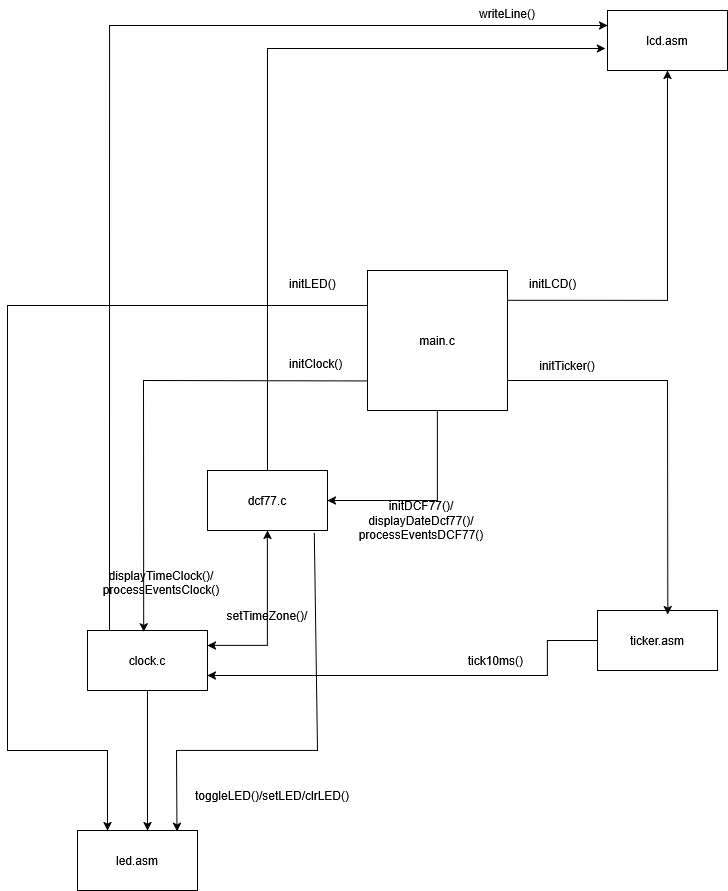
\includegraphics[width=1\textwidth]{diagrams/1.ModuleOverview.png}
    \caption{Module Overview}
    \label{fig:ModuleOverview}
\end{figure}

\newpage

% ---------------------------------------
% 6. Interface Descriptions of All Subroutines
% ---------------------------------------

\section{Interface Descriptions of All Subroutines}

% ---------------------------------------
% 6.1 main.c
% ---------------------------------------

\subsection{main.c}
\begin{itemize}
    \item \textbf{main()}  
    Initializes all modules and calls the corresponding subroutines.
\end{itemize}

% ---------------------------------------
% 6.2 clock.c
% ---------------------------------------

\subsection{clock.c}
\begin{itemize}
    \item \textbf{initClock()}  
    Initializes the clock module and displays the initial time on the LCD.

    \item \textbf{tick10ms()}  
    Called every 10\,ms by the system timer. Updates internal time base, detects full seconds, handles LED toggling, and samples the DCF77 signal.

    \item \textbf{processEventsClock(clockEvent)}  
    Called once per second (on SECONDTICK). Advances the internal clock time (hours, minutes, seconds).

    \item \textbf{setClock(hours, minutes, seconds)}  
    Sets the internal clock time. Resets the tick counter if seconds are set to 0.

    \item \textbf{displayTimeClock()}  
    Displays the current time on the LCD. Prefixes with "US" or "DE" depending on the selected time zone.

    \item \textbf{time()}  
    Returns the CPU uptime in milliseconds since system start.
\end{itemize}



% ---------------------------------------
% 6.3 dcf77.c
% ---------------------------------------

\subsection{dcf77.c}
\begin{itemize}
    \item \textbf{initializePort()}  
    Configures Port H.0 as input to receive the DCF77 signal. Interrupts are disabled.

    \item \textbf{readPort()}  
    Reads the signal level from Port H.0. Returns 0 if LOW, 1 if HIGH.

    \item \textbf{initDCF77()}  
    Initializes the DCF77 module. Sets the initial clock and displays the decoded date on the LCD.

    \item \textbf{displayDateDcf77()}  
    Formats and displays the decoded date on the second line of the LCD.

    \item \textbf{sampleSignalDCF77(currentTime)}  
    Called every 10\,ms to sample the DCF77 signal. Detects falling and rising edges and determines whether the signal represents a valid second, bit, or minute.

    \item \textbf{processEventsDCF77(event)}  
    Processes DCF77 events. Stores received bits, handles complete minute frames, and triggers clock update and date display if valid data is received.

    \item \textbf{eventMinute()}  
    Parses a full DCF77 minute frame. Extracts and validates date and time values, including parity checks. Updates internal variables if successful.

    \item \textbf{USDE()}  
    Applies a \texttt{+6h} or \texttt{-6h} offset to switch between DE and US time zones. Adjusts weekday and date accordingly.

    \item \textbf{USDE\_Pressed()}  
    Checks if the button on Port H.3 is pressed. Toggles the selected time zone and updates display and internal time accordingly.

    \item \textbf{isLeap(year)}  
    Determines whether the given year is a leap year. Returns 1 if true, 0 otherwise.

    \item \textbf{daysInMonth(month, year)}  
    Returns the number of days in the specified month. Accounts for leap years in February.

    \item \textbf{adjustDate(day, month, year, deltaDays)}  
    Adds or subtracts days to a given date, correctly wrapping over month and year boundaries. Used when switching time zones across midnight.
\end{itemize}



% ---------------------------------------
% 6.4 lcd.asm
% ---------------------------------------

\subsection{lcd.asm}
\begin{itemize}
    \item \textbf{initLCD()}  
    Initializes the LCD display. Configures ports, sends initialization command sequences, and clears the display. Must be called once before using the display.

    \item \textbf{writeLine(X, B)}  
    Writes a zero-terminated string to the specified LCD row.  
    \texttt{X} is a pointer to the string, and \texttt{B} is the row number (0 or 1).  
    If the string is shorter than 16 characters, the remaining space is filled with blanks. Longer strings are truncated.

    \item \textbf{delay\_10ms()}  
    Delays execution for approximately 10 milliseconds. Used for timing synchronization during LCD operations.
\end{itemize}


% ---------------------------------------
% 6.5 led.asm
% ---------------------------------------

\subsection{led.asm}
\begin{itemize}
    \item \textbf{initLED()}  
    Initializes the LED output pins. Configures Port B as output and turns off all LEDs. Also activates LED control by enabling Port J.1 and (optionally) disables the seven-segment display.

    \item \textbf{toggleLED(bitmask)}  
    Toggles the state of LEDs specified by the bitmask. A bit set to 1 in the mask inverts the current LED state.

    \item \textbf{setLED(bitmask)}  
    Turns on the LEDs specified by the bitmask. Only bits set to 1 in the bitmask are affected.

    \item \textbf{clrLED(bitmask)}  
    Turns off the LEDs specified by the bitmask. Only bits set to 1 in the bitmask are affected.
\end{itemize}


\newpage

% ---------------------------------------
% 7. Flow Charts
% ---------------------------------------

\section{Flow Charts}

% ---------------------------------------
% 7.1 Main
% ---------------------------------------

\subsection{Main}

\begin{figure}[H]
    \centering
    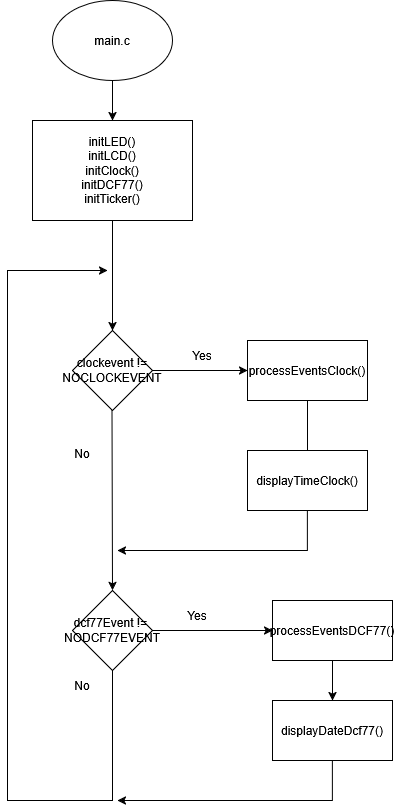
\includegraphics[width=0.6\textwidth]{diagrams/2.Main.png}
    \caption{Main}
    \label{fig:Main}
\end{figure}

% ---------------------------------------
% 7.2 Clock
% ---------------------------------------

\subsection{Clock}

\begin{figure}[H]
    \centering
    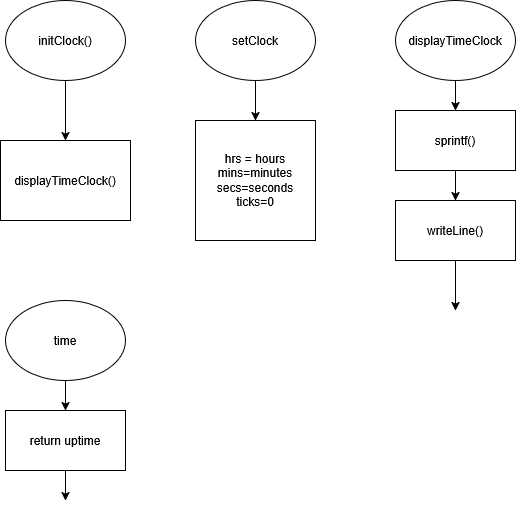
\includegraphics[width=1\textwidth]{diagrams/3.clock1.png}
    \caption{Clock 1}
    \label{fig:Clock1}
\end{figure}

\begin{figure}[H]
    \centering
    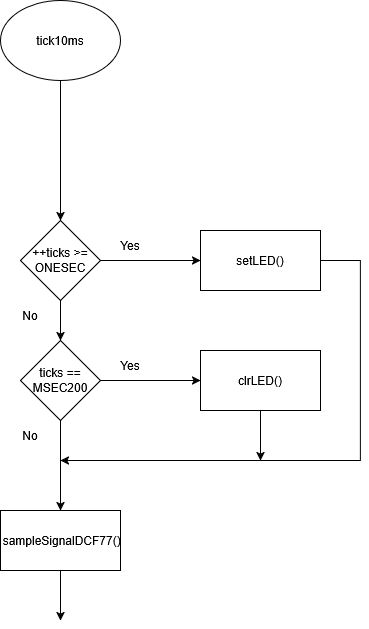
\includegraphics[width=0.8\textwidth]{diagrams/4.clock2.png}
    \caption{Clock 2}
    \label{fig:Clock2}
\end{figure}

% ---------------------------------------
% 7.3 DCF77
% ---------------------------------------

\subsection{DCF77}

\begin{figure}[H]
    \centering
    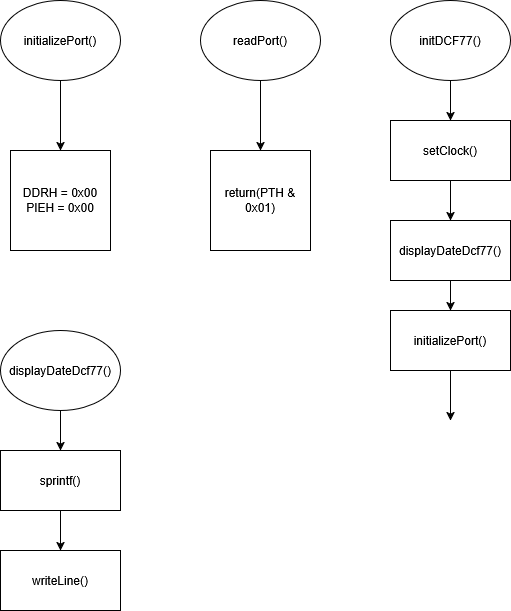
\includegraphics[width=0.8\textwidth]{diagrams/5.dcf771.png}
    \caption{DCF77 - Part 1}
    \label{fig:DCF77}
\end{figure}

\begin{figure}[H]
    \centering
    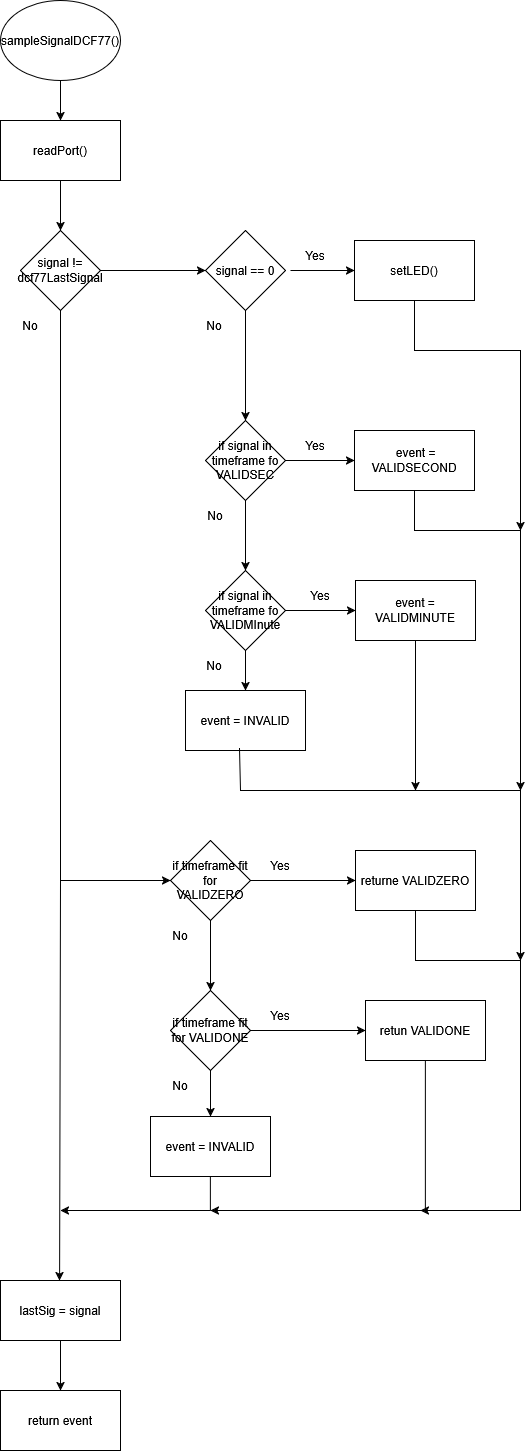
\includegraphics[width=0.525\textwidth]{diagrams/6.dcf772.png}
    \caption{DCF77 - Part 2}
    \label{fig:DCF772}
\end{figure}

\begin{figure}[H]
    \centering
    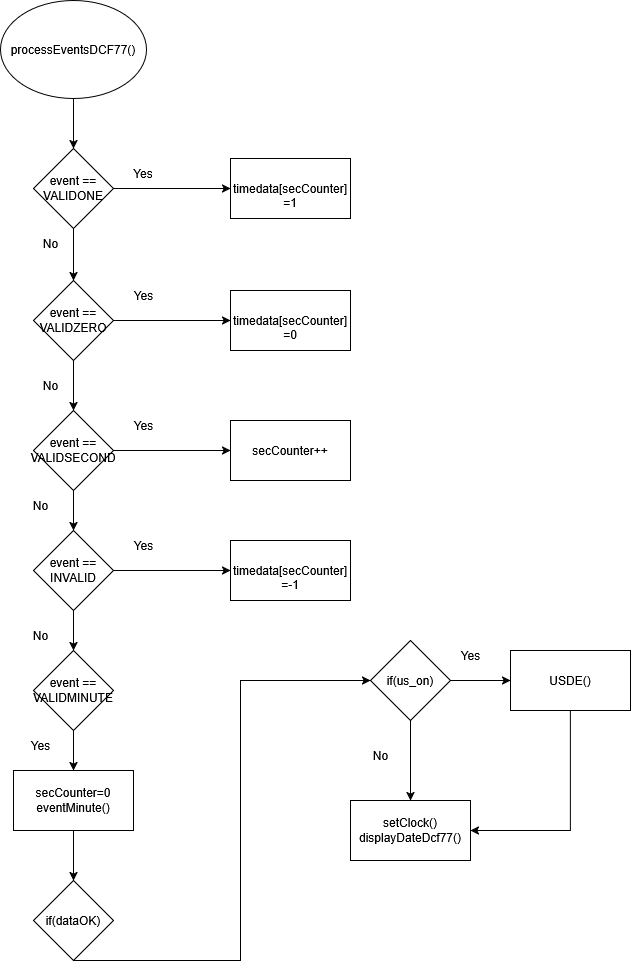
\includegraphics[width=0.95\textwidth]{diagrams/7.dcf773.png}
    \caption{DCF77 - Part 3}
    \label{fig:DCF773}
\end{figure}

\begin{figure}[H]
    \centering
    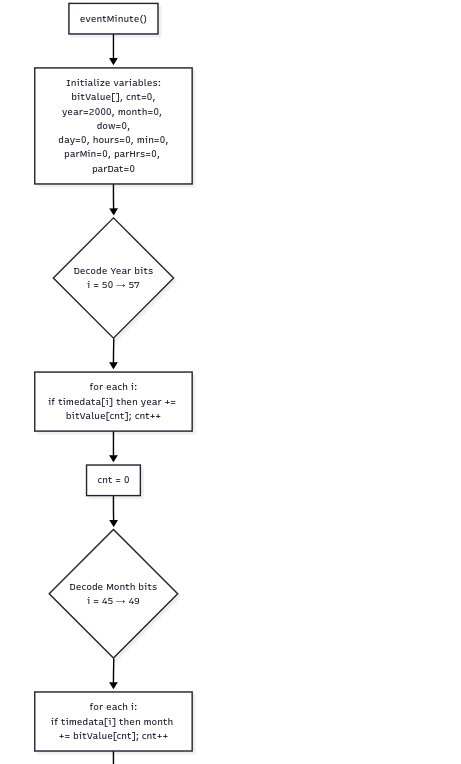
\includegraphics[width=0.7\textwidth]{diagrams/eventMinute/eventMinute1.png}
    \caption{Event Minute – Part 1}
    \label{fig:eventMinute1}
\end{figure}

\begin{figure}[H]
    \centering
    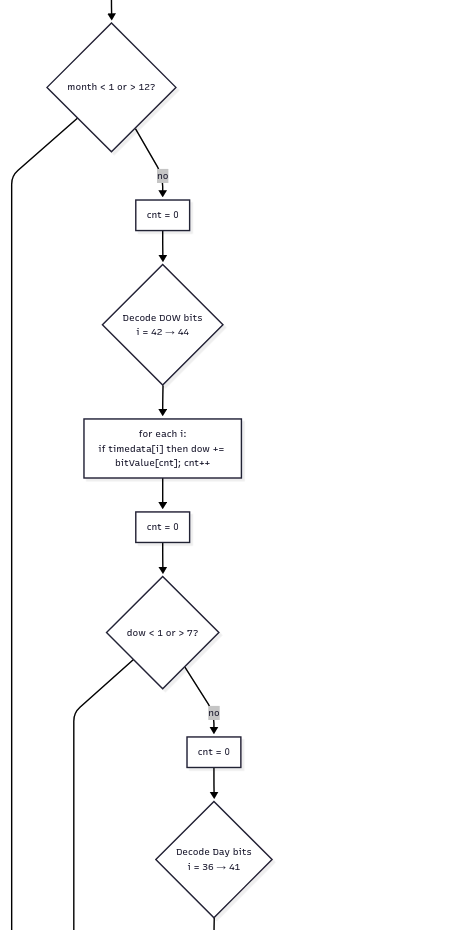
\includegraphics[width=0.7\textwidth]{diagrams/eventMinute/eventMinute2.png}
    \caption{Event Minute – Part 2}
    \label{fig:eventMinute2}
\end{figure}

\begin{figure}[H]
    \centering
    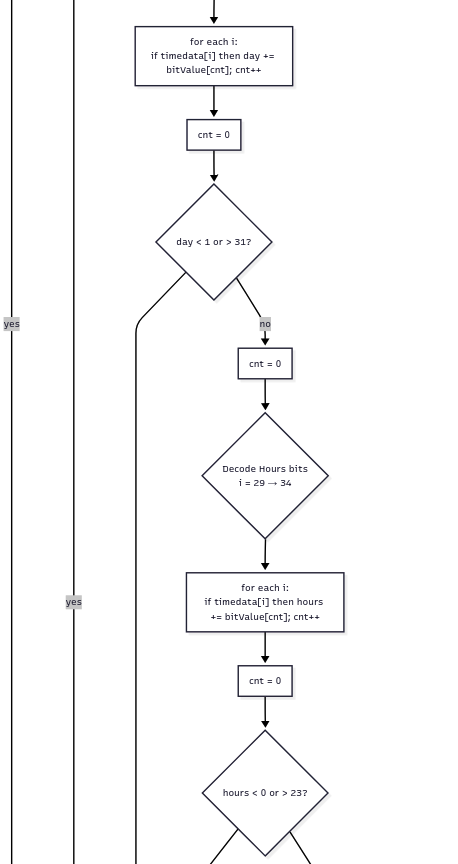
\includegraphics[width=0.7\textwidth]{diagrams/eventMinute/eventMinute3.png}
    \caption{Event Minute – Part 3}
    \label{fig:eventMinute3}
\end{figure}

\begin{figure}[H]
    \centering
    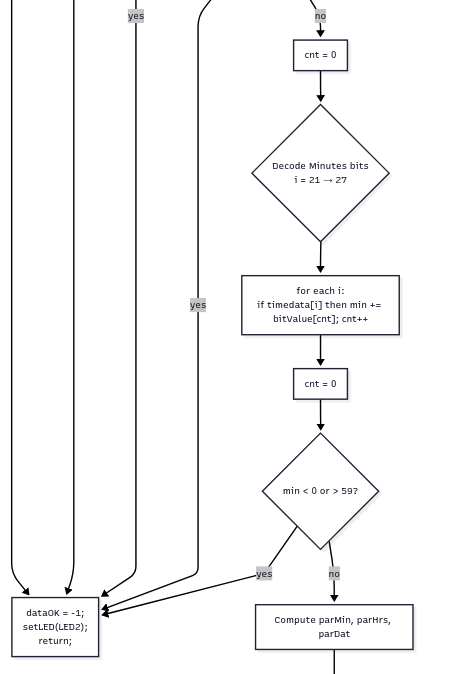
\includegraphics[width=0.7\textwidth]{diagrams/eventMinute/eventMinute4.png}
    \caption{Event Minute – Part 4}
    \label{fig:eventMinute4}
\end{figure}

\begin{figure}[H]
    \centering
    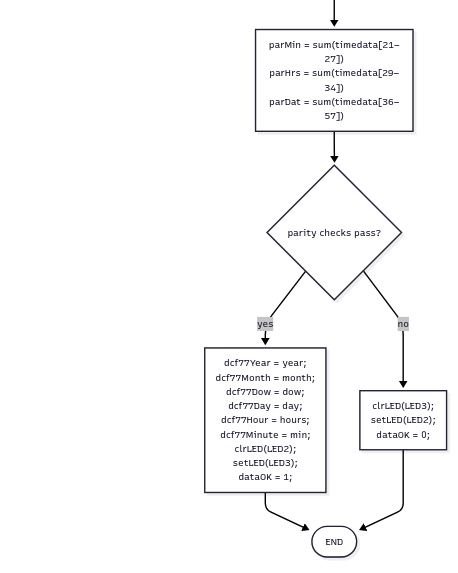
\includegraphics[width=0.7\textwidth]{diagrams/eventMinute/eventMinute5.png}
    \caption{Event Minute – Part 5}
    \label{fig:eventMinute5}
\end{figure}

\begin{figure}[H]
    \centering
    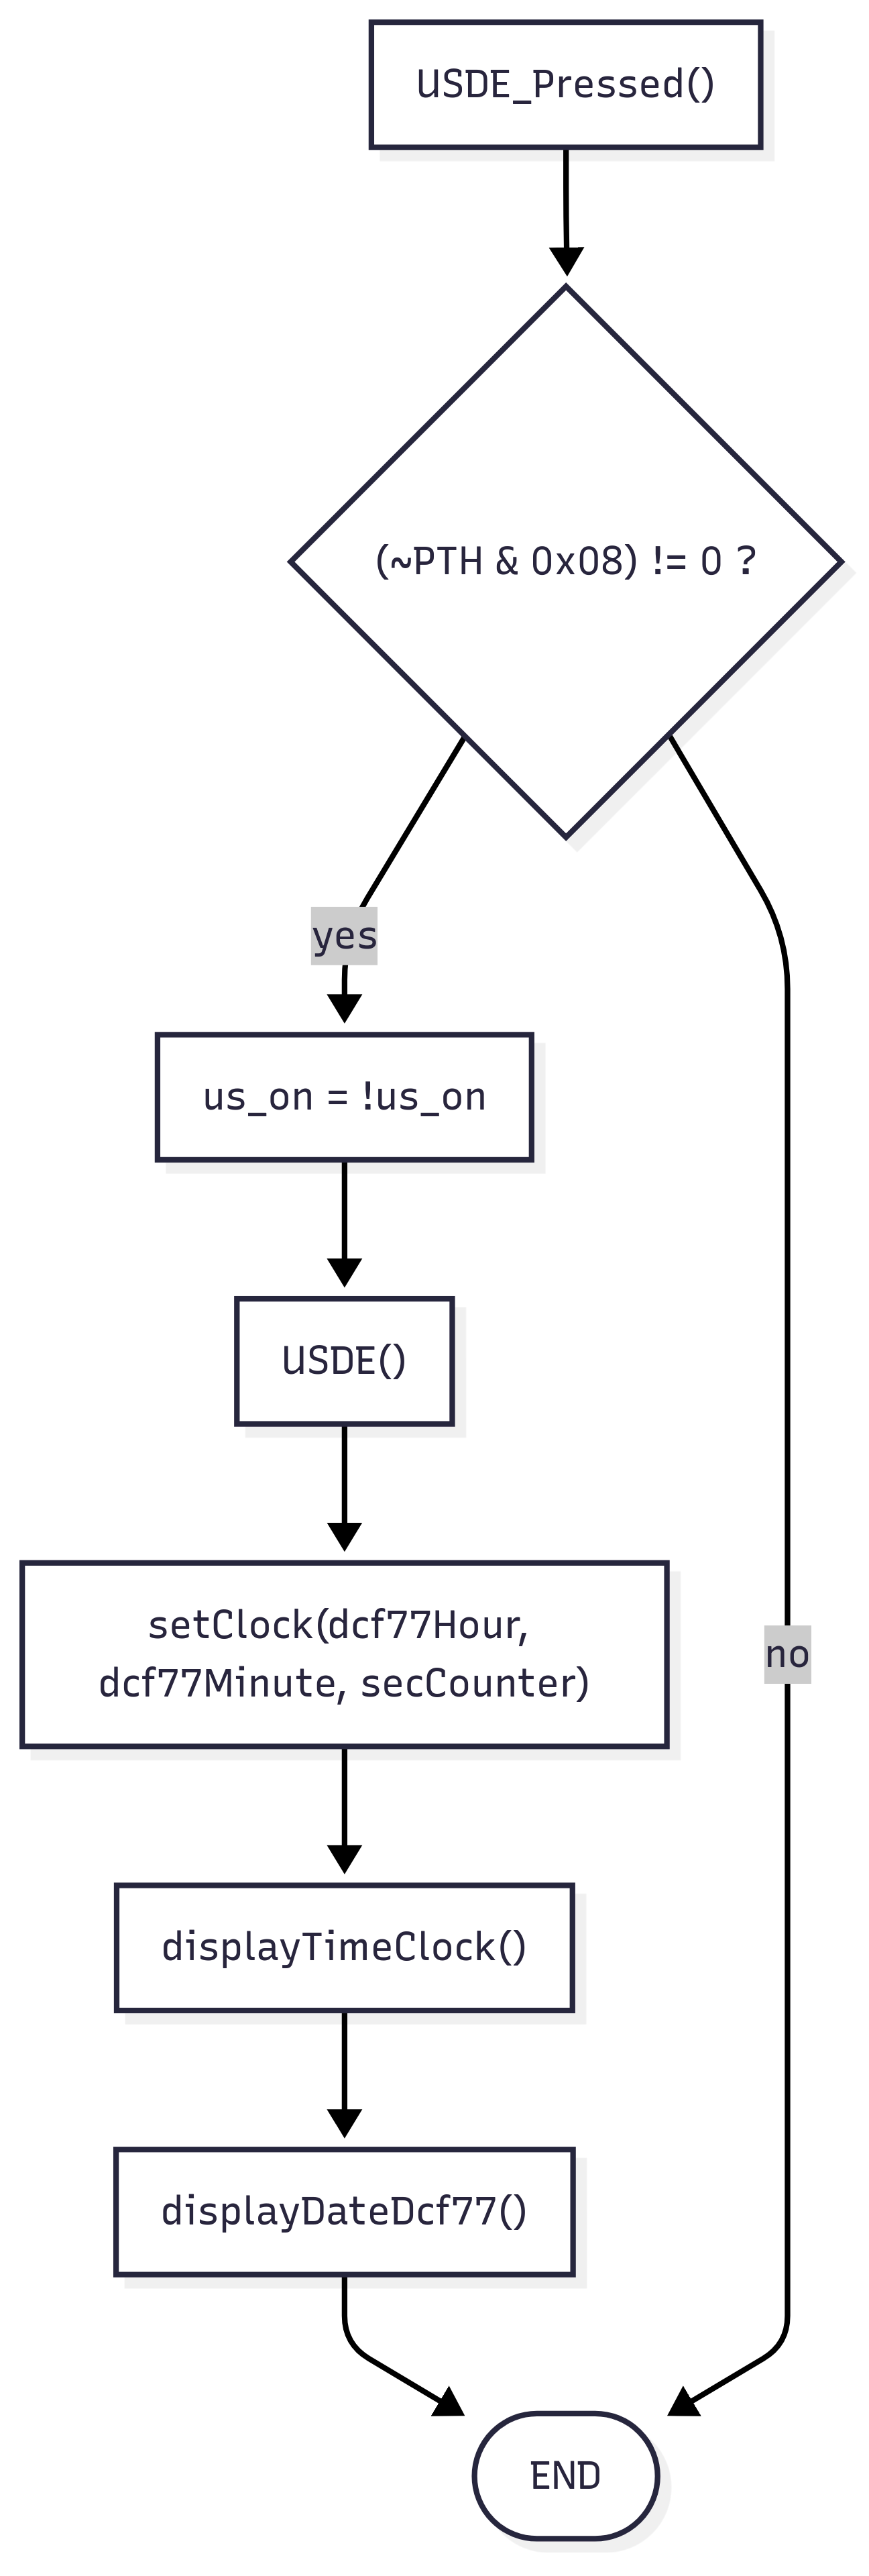
\includegraphics[width=0.45\textwidth]{diagrams/9.USDE_Pressed.png}
    \caption{USDE Pressed}
    \label{fig:USDEPressed}
\end{figure}

\begin{figure}[H]
    \centering
    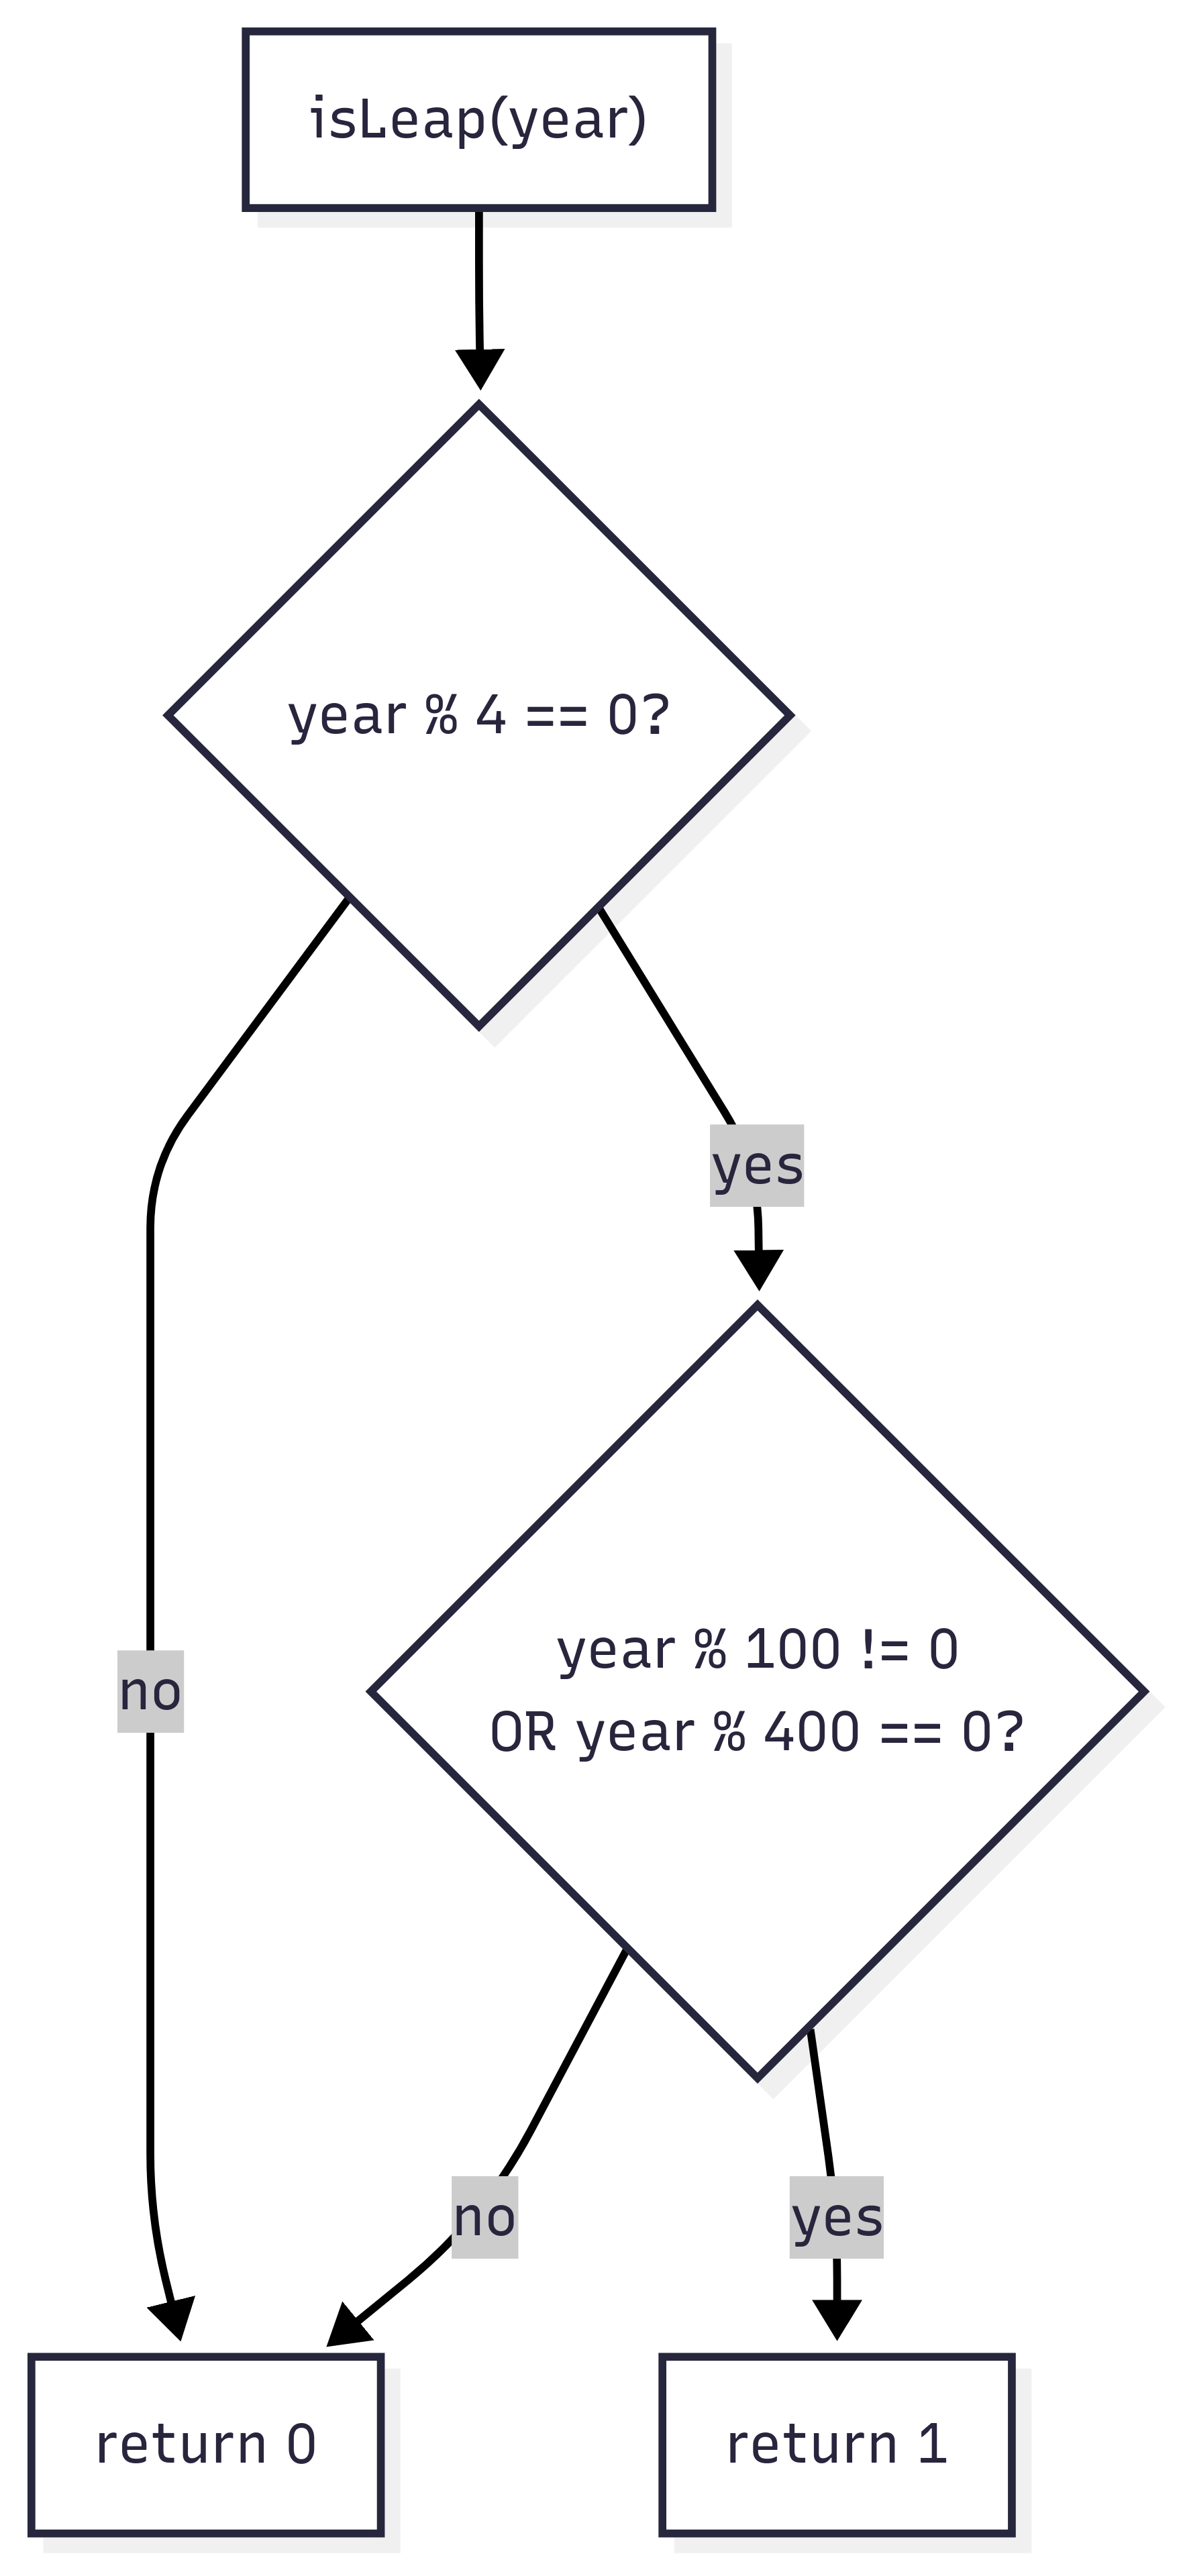
\includegraphics[width=0.5\textwidth]{diagrams/10.isLeap.png}
    \caption{isLeap}
    \label{fig:isLeap}
\end{figure}

\begin{figure}[H]
    \centering
    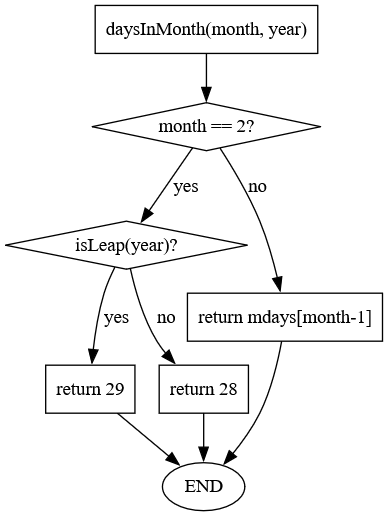
\includegraphics[width=0.7\textwidth]{diagrams/11.daysInMonth.png}
    \caption{daysInMonth}
    \label{fig:daysInMonth}
\end{figure}

\begin{figure}[H]
    \centering
    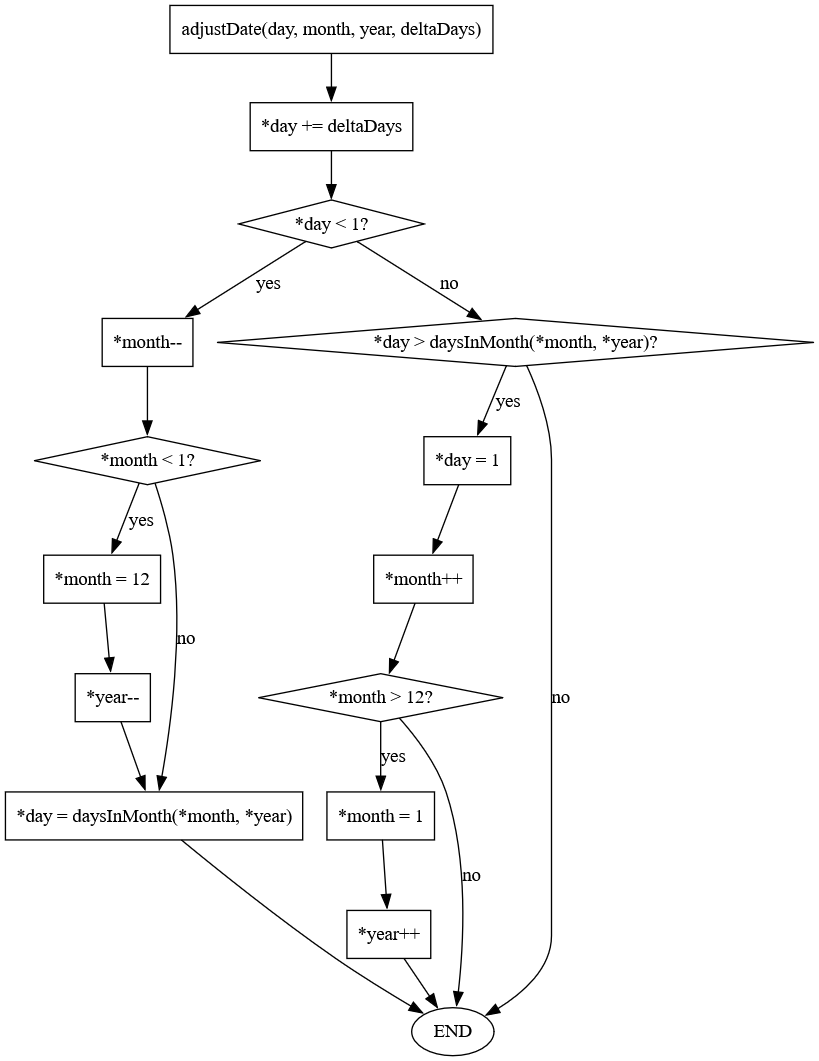
\includegraphics[width=0.9\textwidth]{diagrams/12.adjustDate.png}
    \caption{adjustDate}
    \label{fig:adjustDate}
\end{figure}

\begin{figure}[H]
    \centering
    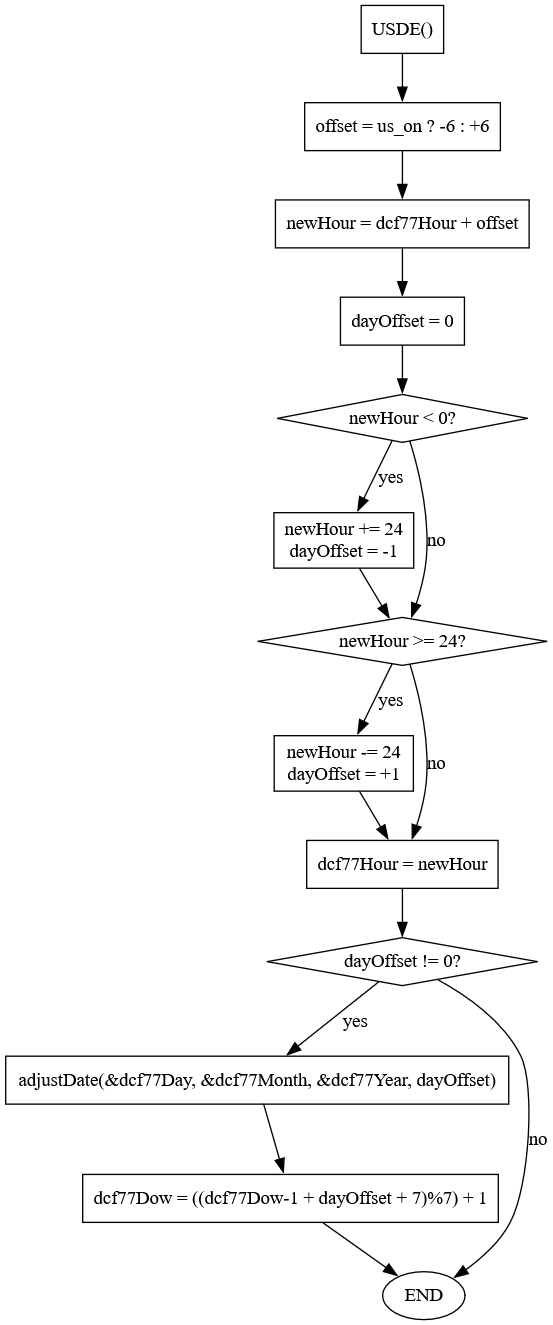
\includegraphics[width=0.55\textwidth]{diagrams/13.USDE.png}
    \caption{USDE}
    \label{fig:USDE}
\end{figure}

\end{document}
